\section{Einleitung}\label{kap:einleitung}

Maschinen bestehen aus mehreren Komponenten und sind anschließend Teil eines großen Systems.
Um zu gewährleisten, dass das System korrekt funktioniert und möglichst selten ausfällt, wird der Zustand mittels Überwachungssystemen möglichst genau ermittelt.
Die Grundlage unterschiedlicher Analyseverfahren sind die aufgenommenen Systemdaten.
Ein wesentlicher Teil davon sind Sensordaten, welche kontinuierlich in Datenspeichern abgelegt und weiterverarbeitet werden.

In einem großen System fallen durch kontinuierliche Datenaufnahme große Datenmengen an.
Um schon preventiv Maschinenausfälle zu vermeiden werden diese Daten weiterverarbeitet und anschließend in Form von Diagrammen, Ampelsystemen, oder ähnlichem visualisiert und für den Menschen lesbar dargestellt.
Es ist Beispielsweise die Rede von \enquote{Condition-Monitoring}. 

Um noch mehr Informationen aus diesen Daten zu erhalten werden unterschiedliche Analyseverfahren angewendet um Anomalien festzustellen und auf diese anschließend zu reagieren.
Eine \enquote{prädektive Instanthaltung} wired dann möglich, wenn diese Anomalien schon vorzeitig erkannt werden.

Die Herausforderung dabei ist der kontinuierliche Datenfluss.
Die Daten müssen, ähnlich zur Livedatenanalyse, direkt verarbeitet werden.
Das hohe Datenvorkommen und die Korrelation der einzelnen Daten macht diese Analyse sehr komplex.
Nähere Zusammenhänge innerhalb der Daten oder sogar zwischen mehrere Datenpaketen zu erkennen ist sehr Rechenaufwändig.
Betracht man mehere Daten innerhalb eines Zeitfensters, dann können diese Daten mittels Approximationen wie in Abbilding\ \ref{fig:FFETimeSeries} (a), (b) und (c) verglichen werden. 
Die Zeitreihendaten sehen in diesem Fall für Menschen nahezu gleich aus. 
Die Approximation kann je nach Datenkomplexität sehr Rechenaufwändig werden und in diesem Fall ist der Informationsgewinn sehr eingeschränkt.
Durch Anwenden von Analysverfahren kann ein gewisser Unterschied erkannt werden.
In Abbildung\ \ref{fig:FFETimeSeries} (d), wurden die Zeitreihen in einem Merkmalsraum, im englischen \enquote{Feature Space}, dargestellt. 
Zeireihe (a) und (c) sind weiterhin sehr ähnlich.
Zeireihe (b) unterscheidet sich etwas im Vergleich zu (a) und (c). 

\begin{figure}
  \centering
  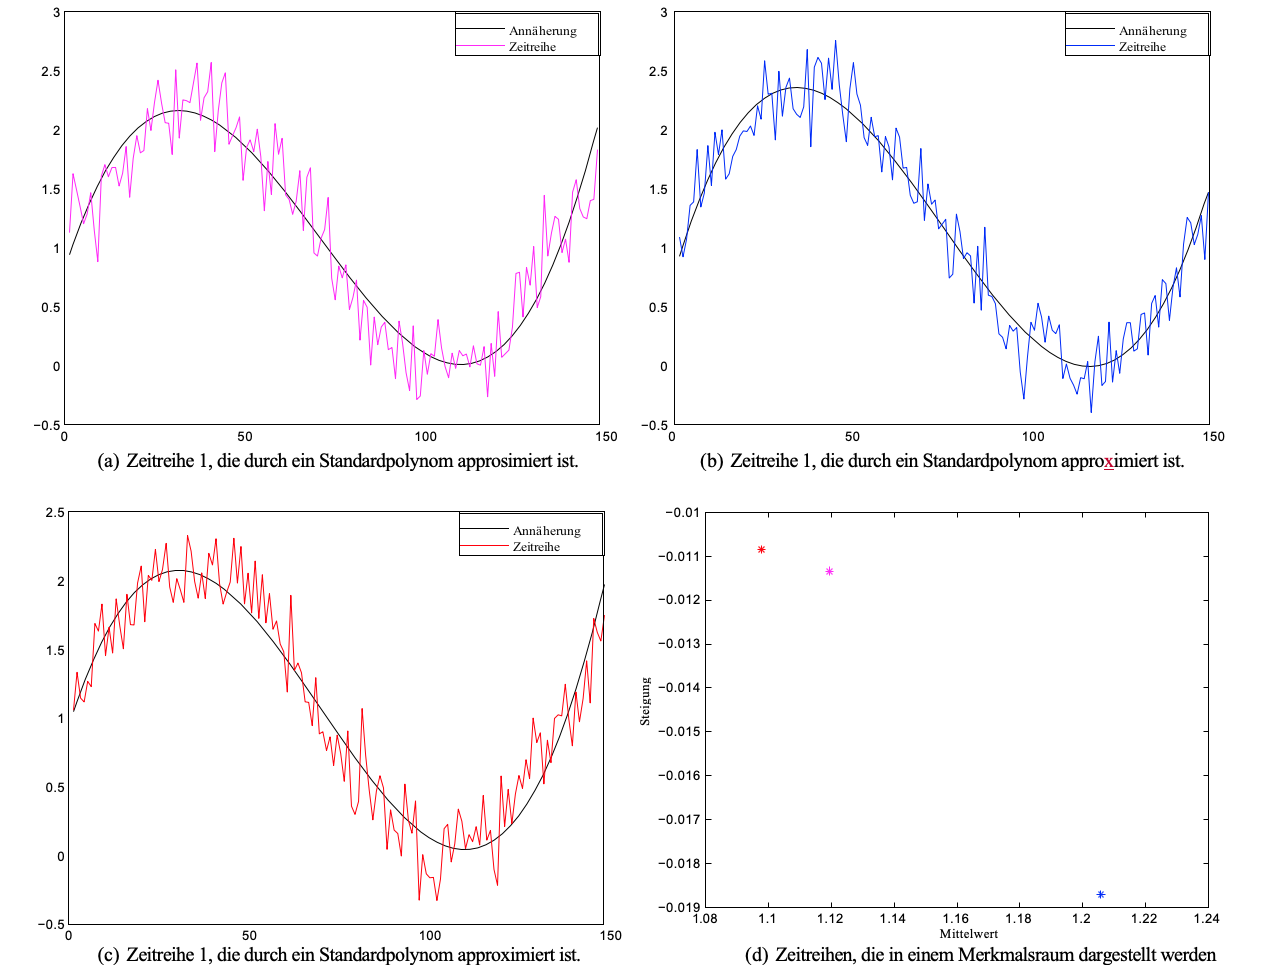
\includegraphics[width=0.9\textwidth]{FastFeatureExtractionTimeSeries.png}
  \caption{Drei standard ploynom Approximationen mittes least-squared. Die Drei Approximationen werden in Abbildung (d) in einem Merkmalsraum dargestellt~\cite{gensler2015fast}.} 
  \label{fig:FFETimeSeries}
\end{figure}

Dieser Merkmalsraum wird durch das Analysieren der Daten auf gewisse Merkmale, im englischen \enquote{Features}, erstellt.
Der Merkmalsraum bietet eine weitere Möglichkeit Daten miteinander zu vergleichen, Anomalien zu erkennen oder die Daten zu klassifizieren. 
Um solche Verfahren anwenden zu können müssen diese Merkmale zuvor extrahiert werden. 
Es ist die Rede von \enquote{Feature Extraktion}.

In diesem Fall handelt es sich um eine polynomielle Approximation der Zeitreihendaten. 
Diese muss in in jedem Zeitschritt für den gewählt Zeitraum neu berechnet werden. 
Dies kann je nach Dimension des zu approximierenden Polynoms sehr Rechenaufwändig und komplex werden.
Bei einer hohen Abtastrate und einer großen Anzahl an Sensoren entstehen rießige Datenmengen, die unter harten Laufzeitbedingungen analysiert werden müssen.
Ein weiterer Vorteil der \enquote{Feature Extraktion} ist das Reduzieren der Komplexität der Daten. Die Daten müssen nicht mehr selbst über polynomielle Modelle analysiert werden, sondern die extrahierten Merkmalen können als Eingabe für die Analyseverfahren dienen. Somit können komplexe polynomielle Datenbilder mithilfe von beispielsweise linearer Verfahren analysiert werden.

In dieser Arbeit wird zu Beginn in Kapitel \ref{kap:grundlagen} die grundlegende Struktur von Sensordaten beschrieben, der Zusammenhang mit Livedaten diskutiert und anschließend die damit verbundene Verwendung von \enquote{Feature Extraktions} Verfahren besprochen. 
In Kapitel \ref{kap:featureextraktion} werden die Randbedingungen und Herausforderungen an Algorithmen zur kontinuierlichen Livedatenanalyse besprochen und Ansätze sowie Algorithmen vorgestellt, die sich mit desem Problemen auseinander setzen.